% Options for packages loaded elsewhere
\PassOptionsToPackage{unicode}{hyperref}
\PassOptionsToPackage{hyphens}{url}
\PassOptionsToPackage{dvipsnames,svgnames,x11names}{xcolor}
%
\documentclass[
]{report}

\usepackage{amsmath,amssymb}
\usepackage{iftex}
\ifPDFTeX
  \usepackage[T1]{fontenc}
  \usepackage[utf8]{inputenc}
  \usepackage{textcomp} % provide euro and other symbols
\else % if luatex or xetex
  \usepackage{unicode-math}
  \defaultfontfeatures{Scale=MatchLowercase}
  \defaultfontfeatures[\rmfamily]{Ligatures=TeX,Scale=1}
\fi
\usepackage{lmodern}
\ifPDFTeX\else  
    % xetex/luatex font selection
\fi
% Use upquote if available, for straight quotes in verbatim environments
\IfFileExists{upquote.sty}{\usepackage{upquote}}{}
\IfFileExists{microtype.sty}{% use microtype if available
  \usepackage[]{microtype}
  \UseMicrotypeSet[protrusion]{basicmath} % disable protrusion for tt fonts
}{}
\makeatletter
\@ifundefined{KOMAClassName}{% if non-KOMA class
  \IfFileExists{parskip.sty}{%
    \usepackage{parskip}
  }{% else
    \setlength{\parindent}{0pt}
    \setlength{\parskip}{6pt plus 2pt minus 1pt}}
}{% if KOMA class
  \KOMAoptions{parskip=half}}
\makeatother
\usepackage{xcolor}
\setlength{\emergencystretch}{3em} % prevent overfull lines
\setcounter{secnumdepth}{-\maxdimen} % remove section numbering
% Make \paragraph and \subparagraph free-standing
\ifx\paragraph\undefined\else
  \let\oldparagraph\paragraph
  \renewcommand{\paragraph}[1]{\oldparagraph{#1}\mbox{}}
\fi
\ifx\subparagraph\undefined\else
  \let\oldsubparagraph\subparagraph
  \renewcommand{\subparagraph}[1]{\oldsubparagraph{#1}\mbox{}}
\fi


\providecommand{\tightlist}{%
  \setlength{\itemsep}{0pt}\setlength{\parskip}{0pt}}\usepackage{longtable,booktabs,array}
\usepackage{calc} % for calculating minipage widths
% Correct order of tables after \paragraph or \subparagraph
\usepackage{etoolbox}
\makeatletter
\patchcmd\longtable{\par}{\if@noskipsec\mbox{}\fi\par}{}{}
\makeatother
% Allow footnotes in longtable head/foot
\IfFileExists{footnotehyper.sty}{\usepackage{footnotehyper}}{\usepackage{footnote}}
\makesavenoteenv{longtable}
\usepackage{graphicx}
\makeatletter
\def\maxwidth{\ifdim\Gin@nat@width>\linewidth\linewidth\else\Gin@nat@width\fi}
\def\maxheight{\ifdim\Gin@nat@height>\textheight\textheight\else\Gin@nat@height\fi}
\makeatother
% Scale images if necessary, so that they will not overflow the page
% margins by default, and it is still possible to overwrite the defaults
% using explicit options in \includegraphics[width, height, ...]{}
\setkeys{Gin}{width=\maxwidth,height=\maxheight,keepaspectratio}
% Set default figure placement to htbp
\makeatletter
\def\fps@figure{htbp}
\makeatother

\makeatletter
\@ifpackageloaded{caption}{}{\usepackage{caption}}
\AtBeginDocument{%
\ifdefined\contentsname
  \renewcommand*\contentsname{Table of contents}
\else
  \newcommand\contentsname{Table of contents}
\fi
\ifdefined\listfigurename
  \renewcommand*\listfigurename{List of Figures}
\else
  \newcommand\listfigurename{List of Figures}
\fi
\ifdefined\listtablename
  \renewcommand*\listtablename{List of Tables}
\else
  \newcommand\listtablename{List of Tables}
\fi
\ifdefined\figurename
  \renewcommand*\figurename{Figure}
\else
  \newcommand\figurename{Figure}
\fi
\ifdefined\tablename
  \renewcommand*\tablename{Table}
\else
  \newcommand\tablename{Table}
\fi
}
\@ifpackageloaded{float}{}{\usepackage{float}}
\floatstyle{ruled}
\@ifundefined{c@chapter}{\newfloat{codelisting}{h}{lop}}{\newfloat{codelisting}{h}{lop}[chapter]}
\floatname{codelisting}{Listing}
\newcommand*\listoflistings{\listof{codelisting}{List of Listings}}
\makeatother
\makeatletter
\makeatother
\makeatletter
\@ifpackageloaded{caption}{}{\usepackage{caption}}
\@ifpackageloaded{subcaption}{}{\usepackage{subcaption}}
\makeatother
\ifLuaTeX
  \usepackage{selnolig}  % disable illegal ligatures
\fi
\usepackage{bookmark}

\IfFileExists{xurl.sty}{\usepackage{xurl}}{} % add URL line breaks if available
\urlstyle{same} % disable monospaced font for URLs
\hypersetup{
  colorlinks=true,
  linkcolor={blue},
  filecolor={Maroon},
  citecolor={Blue},
  urlcolor={Blue},
  pdfcreator={LaTeX via pandoc}}

\author{}
\date{2024-02-20}

\begin{document}

\chapter{Tensor precision / Data
types}\label{tensor-precision-data-types}

These are the common datatypes that are used as of this writing in ML
(usually referred to as \texttt{dtype}):

Floating point formats: - \texttt{fp32} - 32 bits - \texttt{tf32} - 19
bits (NVIDIA Ampere+) - \texttt{fp16} - 16 bits - \texttt{bf16} - 16
bits - \texttt{fp8} - 8 bits (E4M3 and E5M2 formats)

For visual comparison refer to this representations:

\begin{figure}[H]

{\centering 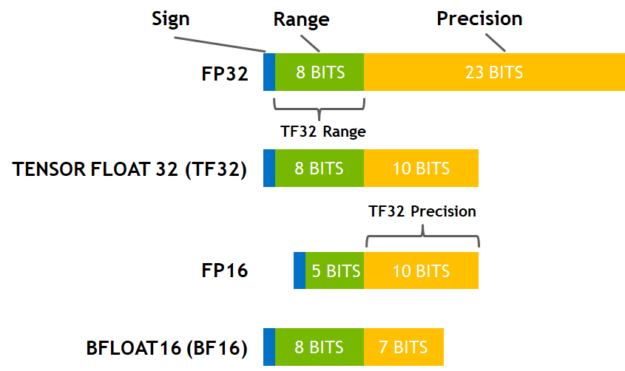
\includegraphics{./images/fp32-tf32-fp16-bf16.png}

}

\caption{fp32-tf32-fp16-bf16}

\end{figure}%

(\href{https://developer.nvidia.com/blog/accelerating-ai-training-with-tf32-tensor-cores/}{source})

\begin{figure}[H]

{\centering 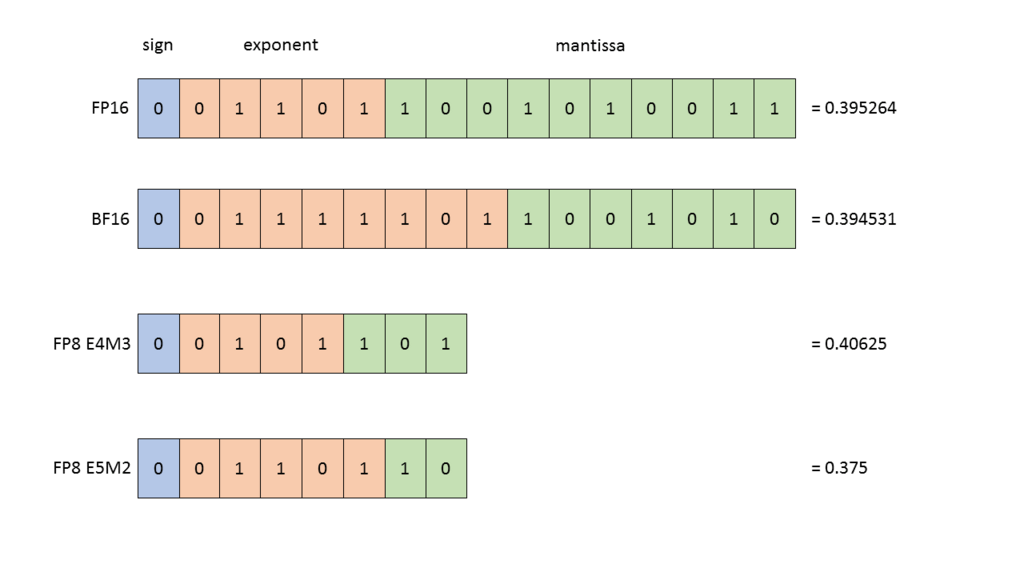
\includegraphics{images/fp16-bf16-fp8.png}

}

\caption{fp16-bf16-fp8}

\end{figure}%

(\href{https://docs.nvidia.com/deeplearning/transformer-engine/user-guide/examples/fp8_primer.html}{source})

Integer formats used in quantization:

\begin{itemize}
\tightlist
\item
  \texttt{int8} - 8 bits
\item
  \texttt{int4} - 4 bits
\item
  \texttt{int1} - 1 bits
\end{itemize}

\section{ML dtype progression}\label{ml-dtype-progression}

Originally ML was using \texttt{fp32}, but it was very slow.

Next
\href{https://developer.nvidia.com/blog/video-mixed-precision-techniques-tensor-cores-deep-learning/}{mixed-precision
was invented using a combination of \texttt{fp16} and \texttt{fp32}} was
invented which tremendously sped up the training speed.

\begin{figure}[H]

{\centering 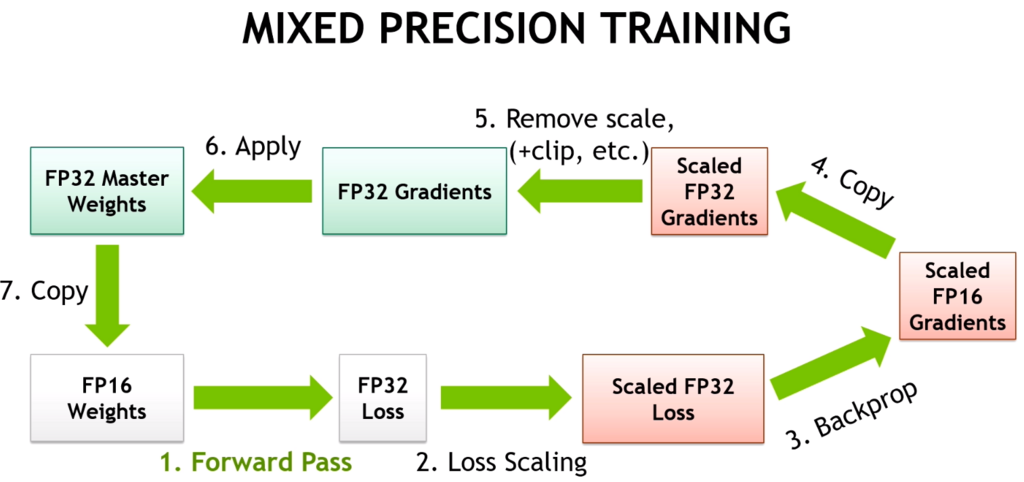
\includegraphics{images/mixed-precision-fp16.png}

}

\caption{fp32/fp16 mixed precision}

\end{figure}%

(\href{https://developer.nvidia.com/blog/video-mixed-precision-techniques-tensor-cores-deep-learning/}{source})

But \texttt{fp16} proved to be not very stable and training LLM was
extremely difficult.

Luckily bf16 came out and replaced \texttt{fp16} using the same mixed
precision protocol. This made the LLM training much more stable.

Then fp8 came and mixed precision has switched to
\href{https://docs.nvidia.com/deeplearning/transformer-engine/user-guide/examples/fp8_primer.html}{that}
and which makes the training even faster. See the paper:
\href{https://arxiv.org/abs/2209.05433}{FP8 Formats for Deep Learning}.

To appreciate the speed ups between the different formats have a look at
this table for NVIDIA A100 TFLOPS spec (w/o sparsity):

\begin{longtable}[]{@{}lr@{}}
\toprule\noalign{}
Data type & TFLOPS \\
\midrule\noalign{}
\endhead
\bottomrule\noalign{}
\endlastfoot
\texttt{fp32} & 19.5 \\
Tensor Float 32 (TF32) & 156 \\
BFLOAT16 Tensor Core & 312 \\
FP16 Tensor Core & 312 \\
FP8 Tensor Core & 624 \\
INT8 Tensor Core & 624 \\
\end{longtable}

Each next dtype is about 2x faster than the previous one (except
\texttt{fp32} which is much slower than the rest).

In parallel with the mixed training regime the ML community starting
coming up with various quantization approaches. Probably one of the best
examples is Tim Dettmers'
\href{https://github.com/TimDettmers/bitsandbytes}{bitsandbytes} which
provides many 4 and 8-bit quantization solutions. The Deepspeed team
also has some
\href{https://www.deepspeed.ai/tutorials/model-compression/}{interesting
quantization solutions}.

\section{TF32}\label{tf32}

TF32 is a magical datatype that is available on NVIDIA GPUs since
Ampere, and which allows \texttt{fp32} \texttt{matmul}s performed at a
much faster speed than normal \texttt{fp32} \texttt{matmul}s with a
small precision loss.

Here is an example of A100 TFLOPS (w/o sparsity):

\begin{longtable}[]{@{}lr@{}}
\toprule\noalign{}
Data type & TFLOPS \\
\midrule\noalign{}
\endhead
\bottomrule\noalign{}
\endlastfoot
\texttt{fp32} & 19.5 \\
Tensor Float 32 (TF32) & 156 \\
\end{longtable}

As you can see TF32 is 8x faster than \texttt{fp32}!

It's disabled by default. To enable it add at the beginning of your
program:

\begin{verbatim}
torch.backends.cuda.matmul.allow_tf32 = True
torch.backends.cudnn.allow_tf32 = True
\end{verbatim}

For more information about the actual precision loss please see
\href{https://pytorch.org/docs/stable/notes/cuda.html\#tensorfloat-32-tf32-on-ampere-and-later-devices}{this}.

\section{\texorpdfstring{When to use \texttt{fp32}
accumulators}{When to use fp32 accumulators}}\label{when-to-use-fp32-accumulators}

Whenever a low-precision dtype is used one has to be careful not to
accumulate intermediary results in that dtype.

\texttt{LayerNorm}-like operations must not do their work in
half-precision, or they may lose a lot of data. Therefore when these
operations are implemented correctly they do efficient internal work in
the dtype of the inputs, but using the \texttt{fp32} accumulation
registers and then their outputs are downcast to the precision of the
inputs.

Generally it's just the accumulation that is done in \texttt{fp32},
since adding up many low-precision numbers is very lossy otherwise.

Here are some examples:

\begin{enumerate}
\def\labelenumi{\arabic{enumi}.}
\tightlist
\item
  Reduction collectives
\end{enumerate}

\begin{itemize}
\item
  \texttt{fp16}: ok to do in \texttt{fp16} if loss scaling is in place
\item
  bf16: only ok in \texttt{fp32}
\end{itemize}

\begin{enumerate}
\def\labelenumi{\arabic{enumi}.}
\setcounter{enumi}{1}
\tightlist
\item
  Gradient accumulation
\end{enumerate}

\begin{itemize}
\tightlist
\item
  best done in \texttt{fp32} for \texttt{fp16} and bf16, but definitely
  is a must for bf16
\end{itemize}

\begin{enumerate}
\def\labelenumi{\arabic{enumi}.}
\setcounter{enumi}{2}
\tightlist
\item
  Optimizer step / Vanishing gradients
\end{enumerate}

\begin{itemize}
\item
  when adding a tiny gradient to a large number, that addition is often
  nullified therefore typically \texttt{fp32} master weights and
  \texttt{fp32} optim states are used.
\item
  \texttt{fp16} master weights and optim states can be used when using
  \href{https://en.wikipedia.org/wiki/Kahan_summation_algorithm}{Kahan
  Summation} or \href{https://en.wikipedia.org/wiki/Rounding}{Stochastic
  rounding} (introduced in
  \href{https://arxiv.org/abs/2010.06192}{Revisiting BFloat16
  Training}).
\end{itemize}

For an example of the latter see:
\href{https://github.com/pytorch/torchdistx/pull/52}{AnyPrecision
optimizer} with the latest version found
\href{https://github.com/facebookresearch/multimodal/blob/6bf3779a064dc72cde48793521a5be151695fc62/torchmultimodal/modules/optimizers/anyprecision.py\#L17}{here}.

\section{Changing precision post
training}\label{changing-precision-post-training}

Sometimes it's OK to change precision after the model was trained.

\begin{itemize}
\item
  Using \texttt{fp16}-pretrained model in bf16 regime usually fails -
  due to overflows (the biggest number that can be represented in
  \texttt{fp16} is 64k) for an indepth discussion and possible
  workaround see this
  \href{https://github.com/huggingface/transformers/pull/10956}{PR}.
\item
  Using bf16-pretrained model in \texttt{fp16} regime usually works - it
  will lose some performance on conversion, but should work - best to
  finetune a bit before using it.
\end{itemize}



\end{document}
